\documentclass{article}

\usepackage{mathrsfs,amsmath}
\usepackage{xcolor}
\usepackage{titlesec}
\usepackage{listings}
\usepackage{syntax}
\usepackage{pythonhighlighting}

\usepackage{graphicx}

\graphicspath{ {./assets/} }

\usepackage[margin=1.4in]{geometry}

\title{Handout \#6 | CS 471} 
\author{Jared Dyreson\\ 
        California State University, Fullerton}

\usepackage [english]{babel}
\usepackage [autostyle, english = american]{csquotes}
\MakeOuterQuote{"}

\titlespacing*{\section}
{0pt}{5.5ex plus 1ex minus .2ex}{4.3ex plus .2ex}
\titlespacing*{\subsection}
{0pt}{5.5ex plus 1ex minus .2ex}{4.3ex plus .2ex}

\usepackage{hyperref}
\hypersetup{
    colorlinks,
    citecolor=black,
    filecolor=black,
    linkcolor=black,
    urlcolor=black
}

\begin{document}

\maketitle
\tableofcontents

\newpage

\section{Questions}

\begin{enumerate}

\item HTTP is known as a stateless protocol. What does this mean?

\begin{itemize}
\item HTTP will execute each request independently. Therefore any past or future requests will not affect the current request.
\end{itemize}

\item What is the difference between HTTP persistent and non-persistent connections?

\begin{itemize}
\item Persistent connections will still have an open TCP connection when the request after the request has been processed. Non-persistent will terminate the connection after.
\end{itemize}

\item What are the advantages and disadvantages of persistent and non-persistent connections?

\begin{itemize}

\item \textbf{Advantages (non-persistent):}

\begin{itemize}
\item Unknown
\end{itemize}

\item \textbf{Disadvantages (non-persistent):}

\begin{itemize}
\item Requires 2 RTTs (round trip time) per object
\item OS overhead for each TCP connection
\item Browsers often open parallel TCP connections to fetch referenced objects
\end{itemize}

\item \textbf{Advantages (persistent):}

\begin{itemize}
\item Takes only one RTT
\item Multiple objects can be sent over a single connection
\end{itemize}

\item \textbf{Advantages (persistent):}

\begin{itemize}
\item Unknown
\end{itemize}

\end{itemize}

\newpage
\item Describe the basic structure of an HTTP request and response

\begin{itemize}
\item A \emph{start-line} describing the requests to be implemented, or its status of whether its successful or a failure
\item An optional set of \emph{HTTP headers} specifying the request, or describing the body included in the message.
\item A blank line indicating all meta-information for the request has been sent
\item An optional \emph{body} containing data associated with the request (like content of an HTML form), or the document associated with a response. The presence of the body and its size is specified by the starting line and HTTP headers.
\item \textbf{NOTE:} more information can be found \href{https://developer.mozilla.org/en-US/docs/Web/HTTP/Messages}{\underline{here}}
\end{itemize}
\begin{figure}[!h]
\centering
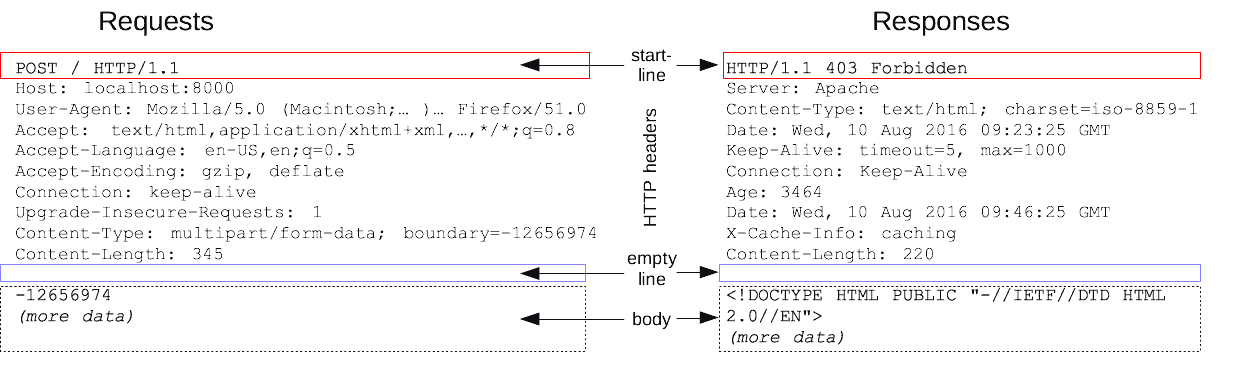
\includegraphics[width=14cm]{HTTP_Request}
\caption{HTTP request}
\end{figure}

\item What is round trip time (RTT)? How many RTTs does it take to fetch a webpage from a server? Explain.

\begin{itemize}
\item \textbf{RTT:} The time (in milliseconds) it takes from the initiating client to issue the request and receive a response.
\item It would take exactly two RTTs; the first GET request and a subsequent response with the webpage
\end{itemize}

\item What is the difference between the HTTP GET and POST methods
\begin{itemize}
\item The GET request will ask the server for some resource
\item The POST request will provide information needed on a given webpage
\end{itemize}

\item What HTTP message fields are used for implementing web cookies?
\begin{itemize}
\item Cookies use the "Set-Cookie" header field
\item More information can be found \href{https://developer.mozilla.org/en-US/docs/Web/HTTP/Cookies}{\underline{here}}
\end{itemize}

\item How long (in terms of RTTs) would it take to retrieve a webpage containing 10 negligibly small images using persistent and non-persistent connections respectively?

\begin{itemize}
\item Persistent: 20 RTTs (this information is found on a Quizlet set, so it can be debated)
\item Non-persistent: 1 RTTs
\end{itemize}

\item What are the two key advantages of web proxies?
\begin{itemize}
\item \textbf{Web Proxy:} an intermediary application between the client and server
\item Reduces response time for client requests and traffic on access links
\end{itemize}
\item Explain the sequence of HTTP messages between the web client, web server, and web proxy server, when fetching a webpage. Be sure to mention the relevant fields in all HTTP messages.
\begin{figure}[!h]
\centering
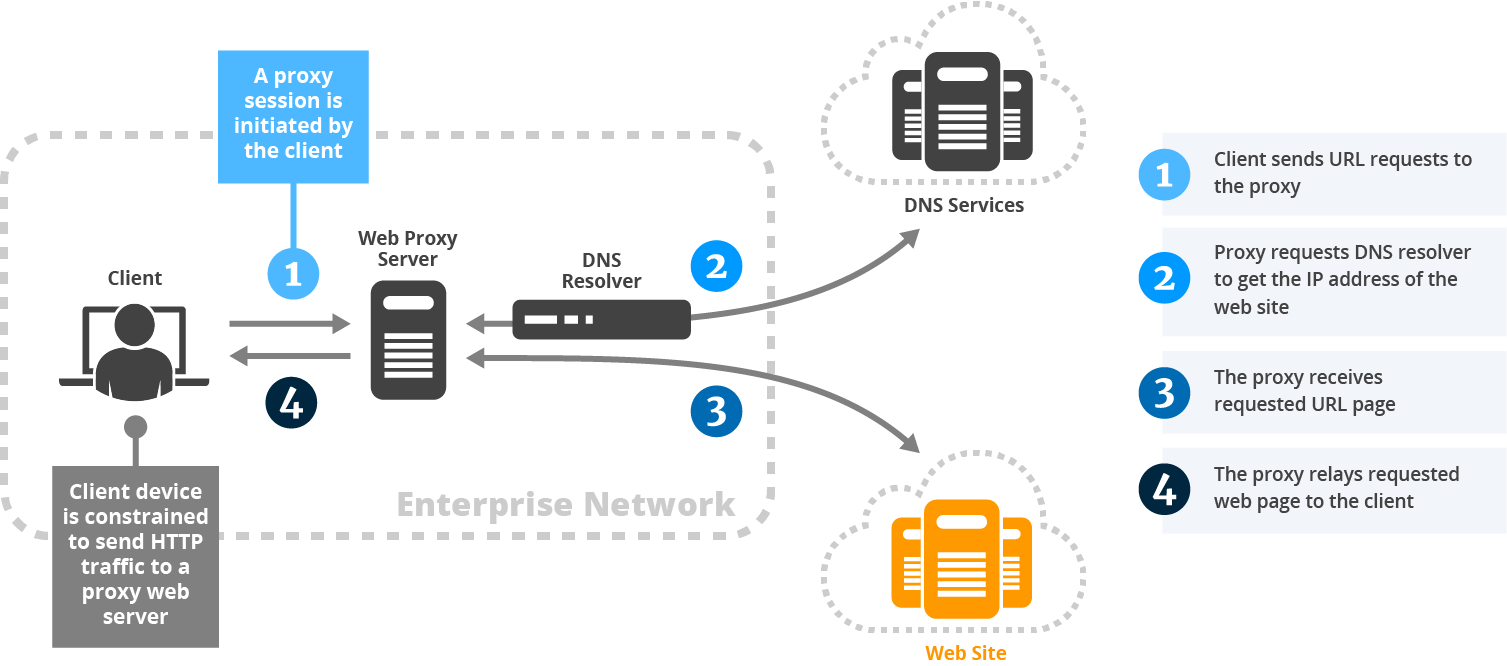
\includegraphics[width=13cm]{Web-Proxy-how-does-it-work}
\end{figure}

\begin{itemize}
\item Client sends request to proxy
\item Proxy will parlay request to the destination
\item The destination server will then give the response to the proxy
\item Proxy will then relay the response to the server
\item \textcolor{red}{I wrote this before reading the diagram in full lol}
\end{itemize}
\end{enumerate}

\end{document}

